%%%%%%%%%%%%%%%%%%%%%%%%%%%%%%%%%%%%%%
\chapter{EFFECTS OF THE EPSILON-NEAR-ZERO TRANSITION LAYER ON THE PROPAGATION OF SURFACE PLASMON POLARITONS}


%%%%%%%%%%%%%%%%%%%%%%%%%%%%%%%%%%%%%%
\section{Introduction}

A~system consisting of dielectric and conducting regions can support a~specific type of electromagnetic excitations --- surface plasmon polaritons (SPPs), --- that are inherently confined in the~vicinity of the~interface between the~two media.
Such excitations propagate in a~self-sustainable manner, where the~electromagnetic field impinging the~conductor (usually a~metal) accelerates the~charges below the~the~metallic surface, and in their turn, the~oscillating charges emit the~coherent radiation back into the~dielectric.
The~amplitudes of both the~charge and the~field oscillations decay exponentially away from the~interface, and for that reason the~SPPs are extremely sensitive to the~surface conditions.
The SPPs find applications in a large number of areas of research and technology, ranging from optoelectronic devices and near-field imaging to tumor treatment and solar cell design \cite{smallworld,notsosmall,schuller}.

The~emergence of metamaterials allowed realization of unconventional material properties in physical devices, which led to the~observation of quite unique electromagnetic phenomena such as, for example, negative index of refraction \cite{veselago,pendry,shalaev2}.
Besides the~possibilities to achieve negative dielectric permittivity and/or magnetic permeability, metamaterials can be engineered to create regions where the refractive index is almost zero \cite{schilling}.
The latter manifests in either sophisticated metal-dielectric compounds or, what is more surprising, even in systems built from the dielectric materials only \cite{moitra}.

While the propagation of electromagnetic waves through such epsilon-near-zero (ENZ) regions has been studied to a certain extent \cite{ginzburg}, it is still of great interest to study the corresponding behavior of the surface plasmons.
Moreover, I will explain in this chapter that a thin ENZ layer always emerges at any metal-dielectric interface which thus qualitatively modifies the SPP properties.
Consequently, one will be able to tune the plasmonic properties by applying an external electrostatic field to the transition layer and thus gaining control over its width.

%%%%%%%%%%%%%%%%%%%%%%%%%%%%%%%%%%%%%%%%%%%%%%%%%%%%%%%%%%%%%%%%%%%%
\section{Metal-Dielectric Interface}

In the~simplest case of the~SPP propagation along the~planar metal-dielectric interface, one typically views the~two media as perfectly uniform materials, with the~boundary between them being a~flat and infinitesimally thin plane.
Naturally, neither the~unavoidable surface roughness of any real experimental sample, nor the~possible material defects or impurities are accounted for in such a~representation. 
The~scattering of the~SPP on the~various types of surface defects is extensively discussed, for example, in the~review \cite{zayats}, so in this chapter, I will restrict the~discussion to the~defect-free scenario, which, however, still allows for a~nontrivial interface structure.

The~material properties, e.g. the~electron density $n$ and the~dielectric permittivity $\epsilon$, must suffer a~discontinuity in the~case of the~ideal interface, which is not physically sound for any real contact between the~two media.
Specifically, on a~microscopic level, the~electrons are confined within the~bulk of the~metal, yet the~essentially quantum nature of their motion presents a~nonzero probability of tunneling through the~potential barrier of the ion lattice, and thus a~sparse cloud of electrons is formed just above the~surface of the~metal.
Together with the~reduced electron population below the~surface of the~metal, this cloud forms a~thin transition layer where the~material properties now change smoothly from their respective values in metal to those in dielectric.
Since the~dielectric constants of the~two media have different signs --- for dielectrics $\epsilon_d > 0$, while for metals $\epsilon_m < 0$ within the~wide range of frequencies, --- a~critical point where $\epsilon = 0$ emerges close to the~surface of the~metal.

\begin{figure}
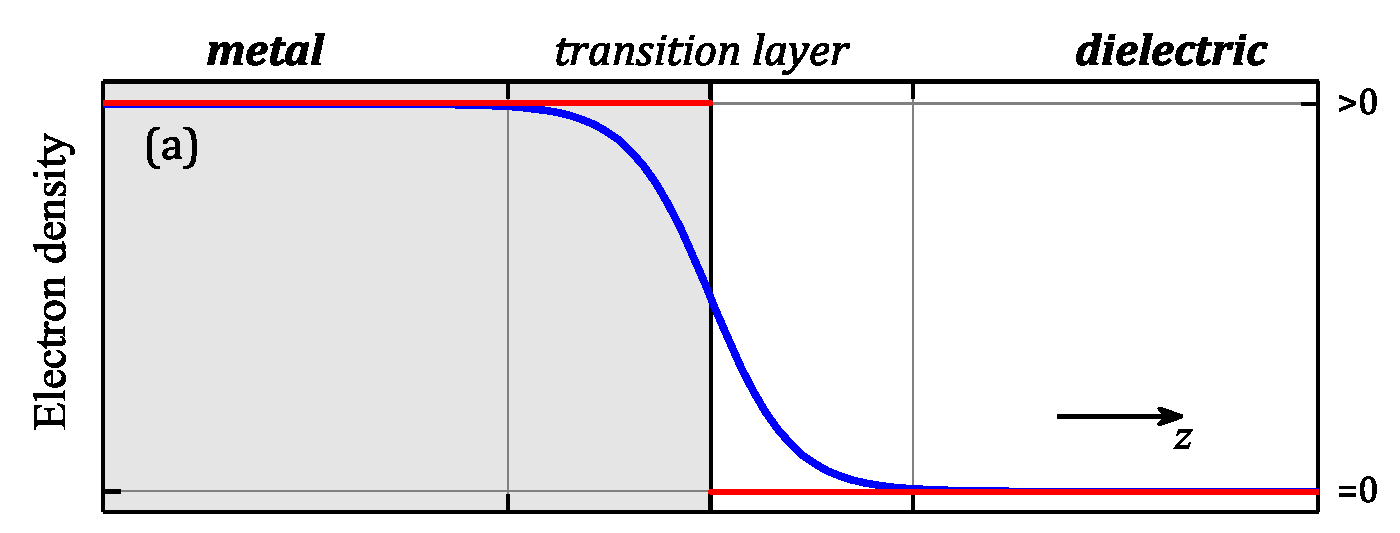
\includegraphics[width=\linewidth]{transitionA.eps}
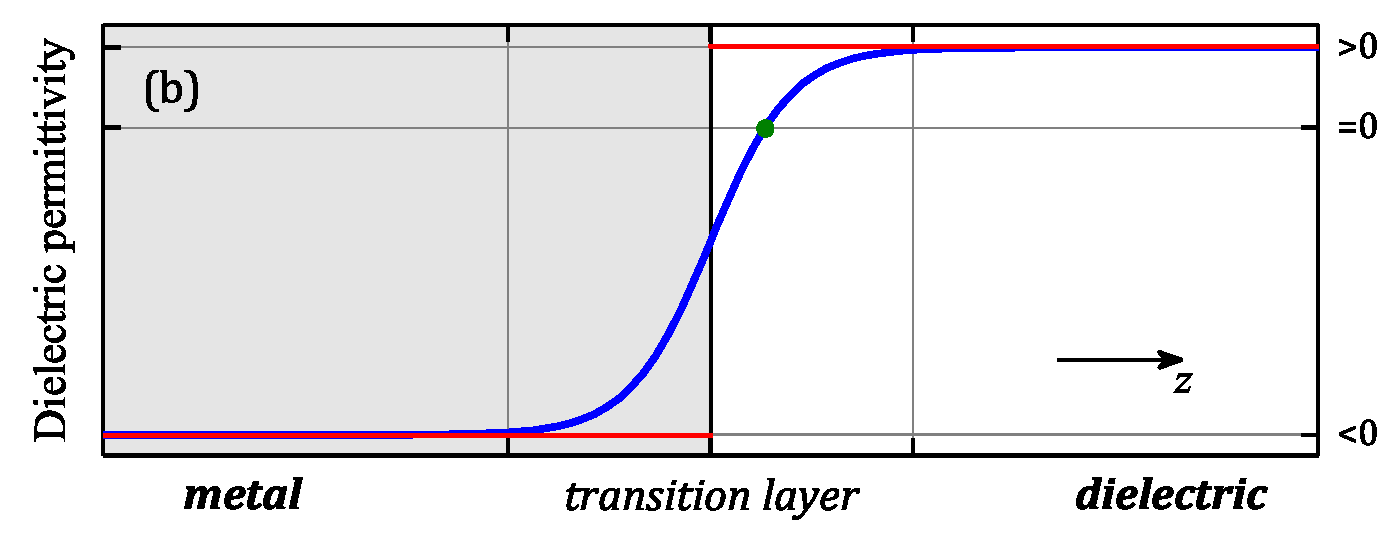
\includegraphics[width=\linewidth]{transitionB.eps}
\caption{Electron density (a) and dielectric permittivity (b) profiles in the vicinity of the metal-dielectric interface. The qualitative behavior for these two quantities is shown assuming the ideally sharp boundary (red lines) and the smooth transition of material properties (blue curves). At some critical point located in the dielectric close to the metal surface, the dielectric permittivity becomes zero (green dot).}
\label{fig:profilePlasmon}
\end{figure}

The~exact solution for the~electron density profile is known to feature the~so-called Friedel oscillations \cite{friedel}, but in this study, I will assume the~electron density to be monotonically decreasing away from metal (see \cref{fig:profilePlasmon}).
This simplification is justified by the~fact that the~qualitative behavior of the~SPP does not depend on the~particular choice of the~electron distribution within the~transition layer (see the~discussion in \cite{prigogine}).
As a result, the analysis presented below does not rely on a particular choice of the dielectric permittivity profile, as opposed to the studies \cite{akimov,gabitov1,gabitov2}, and, moreover, can be generalized to 2D or 3D geometries.

One may also wonder whether the use of macroscopic parameters to describe the ENZ layer is justified at all.
Indeed, the typical size of the transition layer varies from several angstrom to several nanometers \cite{akimov}, which is at least an order of magnitude larger than the characteristic inter-atomic distance in the bulk of the media.
This way the ENZ layer is populated by a sufficient number of spillout electrons, whose collective response to the electromagnetic field is then best described by the macroscopic dielectric permittivity.


%%%%%%%%%%%%%%%%%%%%%%%%%%%%%%%%%%%%%%%%%%%%%%%%%%%%%%%%%%%%%%%%%%%%
\section{Wave Equation for SPP Propagation}

Let us consider a~general case of a~system consisting of dielectric and metallic regions, which alternate along the~$z$-direction and are uniform and isotropic in $x$- and $y$-directions.
In this system, the~dielectric permittivity at any point can be written as $\epsilon = \epsilon(z)$, which may be either continuous or discontinuous function of the~coordinate $z$.

The~electromagnetic field in the~system is a~solution of the~Maxwell's equations:
%
\begin{align}
\nabla \times \mathbf{E} &= -\dfrac{1}{c} \dfrac{\partial \mathbf{H}}{\partial t}, \label{eq:maxwellE} \\
\nabla \times \mathbf{H} &= +\dfrac{1}{c} \dfrac{\partial \mathbf{D}}{\partial t}, \label{eq:maxwellH}
\end{align}
%
where the~electric displacement is $\mathbf{D} = \epsilon \mathbf{E}$, and the~uniform magnetic susceptibility of $\mu = 1$ is assumed.

It is well-known that any plasmonic mode supported by such structure must be a~$p$-polarized (transverse magnetic or TM) wave propagating along the~metal-dielectric interface.
Therefore, without any loss of generality, one may seek the~solutions for the~SPP mode in the~form of a~monochromatic running wave
%
\begin{equation}
\label{eq:runningH}
\mathbf{H} = H_y(z) e^{ikx - i\omega t}\hat{\mathbf{e}}_y,
\end{equation}
%
with the~magnetic field $\mathbf{H}$ being parallel to the~interface between media and perpendicular to the~direction of propagation.
Replacing thus the~time derivative $\partial/\partial t$ with $-i\omega$ and eliminating the~electric field from \cref{eq:maxwellE,eq:maxwellH}, one obtains the~following wave equation:
%
\begin{equation*}
\nabla\times \left( \dfrac{1}{\epsilon} \nabla\times\mathbf{H} \right) = \dfrac{\omega^2}{c^2} \mathbf{H},
\end{equation*}
%
which can be simplified and written down in terms of $H_y(z)$ as
%
\begin{equation}
\label{eq:waveeqPlasmon}
\dfrac{d}{dz}\left(\dfrac{1}{\epsilon(z)}\dfrac{dH_y}{dz}\right) + \left(\dfrac{\omega^2}{c^2}-\dfrac{k^2}{\epsilon(z)}\right)H_y(z) = 0.
\end{equation}
%
This is the~well-known equation for the~$p$-polarized electromagnetic waves propagating in a~nonuniform medium \cite{LLtom8}.
The~subscript "$y$" will be omitted everywhere below as the~magnetic field will be assumed to always point along the~$y$-axis.

\section{SPP Dispersion and Field Profiles: Ideal Case}

Before addressing the~SPP propagation problem along the~transition layer, I will briefly summarize the~main properties that are distinct to the~SPP propagating along the~sharp boundary.
As will be seen further, knowing the SPP magnetic field distribution and its dispersion in the case of ideal boundary allows one to analytically calculate the SPP dispersion corrections due to the presence of the transition layer.


\subsection{Single-Interface System}

In the~case of a~discontinuous dielectric function profile
\begin{equation}
\label{eq:idealeps1Plasmon}
\epsilon_0(z)~=~\left[
\begin{aligned}
&\epsilon_d, &z>0,\\
&\epsilon_m, &z<0,
\end{aligned}
\right.
\end{equation}
which describes an~ideal interface between metallic ($\epsilon_m<0$) and dielectric ($\epsilon_d>0$) semi-spaces, the~plasmonic solution of the~wave equation \cref{eq:waveeqPlasmon} is well-known \cite{zayats}:
\begin{equation}
\label{eq:idealeps1HfieldPlasmon}
H_0(z)~=~H_0 \times \left[
\begin{aligned}
&e^{-\kappa_d z}, &z>0,\\
&e^{+\kappa_m z}, &z<0,\\
\end{aligned}
\right.
\end{equation}
where $\kappa_{d,m} = \sqrt{k^2-\epsilon_{d,m}\omega^2/c^2}$, and the~SPP dispersion $\omega=\omega_0(k)$ is given by
\begin{equation}
\label{eq:idealeps1dispPlasmon_2}
\frac{\epsilon_m}{\epsilon_{d}}\frac{\kappa_{d}}{\kappa_m}+1~=~0
\end{equation}
or
\begin{equation}
\label{eq:idealeps1dispPlasmon}
k~=~\frac{\omega}{c}\sqrt{\frac{\epsilon_d\epsilon_m}{\epsilon_d+\epsilon_m}}.
\end{equation}

Note that in order to solve the~wave equation with the~discontinuous dielectric function, the~boundary conditions for both magnetic and longitudinal electric fields must hold, namely, the~functions $H_0(z)$ and $\epsilon_0^{-1}(z)\dfrac{dH_0}{dz}$ must be continuous.

From now on, the~quantities with the~subscript "$0$" will be describing the~SPP properties in cases with ideal boundaries.



\subsection{Double-Interface System}

In the~case of a~discontinuous dielectric function profile
\begin{equation}
\label{eq:idealeps2Plasmon}
\epsilon_0(z)~=~\left[
\begin{aligned}
&\epsilon_{d+}, &z>+s,\\
&\epsilon_m, &|z|<s, \\
&\epsilon_{d-}, &z<-s,
\end{aligned}
\right.
\end{equation}
which corresponds to a~metal film of thickness $2s$ clad between two different bulk dielectrics (with permittivities $\epsilon_{d+}$ and $\epsilon_{d-}$, respectively), the~SPP dispersion is implicitly given \cite{zayats} by the~following equation:
\begin{equation}
\label{eq:idealeps2dispPlasmon}
\left(\frac{\epsilon_m}{\epsilon_{d+}}\frac{\kappa_{d+}}{\kappa_m}+1\right)\left(\frac{\epsilon_m}{\epsilon_{d-}}\frac{\kappa_{d-}}{\kappa_m}+1\right)~=~\left(\frac{\epsilon_m}{\epsilon_{d+}}\frac{\kappa_{d+}}{\kappa_m}-1\right)\left(\frac{\epsilon_m}{\epsilon_{d-}}\frac{\kappa_{d-}}{\kappa_m}-1\right) e^{-4\kappa_m s}.
\end{equation}
Its solutions represent coupled modes, meaning that the~SPP on one interface is intertwined with that on the~other interface due to the~small thickness of the~film.
For a~sufficiently thick metal film, however, $s \rightarrow \infty$, the~dispersion relation \cref{eq:idealeps2dispPlasmon} naturally decouples into two:
\begin{equation}
\frac{\epsilon_m}{\epsilon_{d\pm}}\frac{\kappa_{d\pm}}{\kappa_m}+1~=~0,
\end{equation}
which separately describe plasmonic modes existing independently on each interface (see the~dispersion equation \cref{eq:idealeps1dispPlasmon_2})

As for the~SPP magnetic field, I write it down as follows:
\begin{equation}
\label{eq:idealeps2HfieldPlasmon}
H_0(z)~=~H_0 \times \left[
\begin{aligned}
&\CA e^{-\kappa_{d+} (z-s)}, &z>+s,\\
&\CB e^{+\kappa_m z} + \CC e^{-\kappa_m z}, &|z|<s,\\
&\CD e^{+\kappa_{d-} (z+s)}, &z<-s,\\
\end{aligned}
\right.
\end{equation}
where the~coefficients $\CA$, $\CB$, $\CC$ and $\CD$ are related through the~boundary conditions at the~interfaces $z=\pm s$.
The~continuity of $H_0(z)$ and $\epsilon_0^{-1}(z)\dfrac{dH_0}{dz}$ yields
\begin{align}
\CA~=~\CB e^{+\kappa_m s} + \CC e^{-\kappa_m s},& \qquad
-\frac{\kappa_{d+}}{\epsilon_{d+}}\CA~=~\frac{\kappa_m}{\epsilon_m}\left(\CB e^{+\kappa_m s} - \CC e^{-\kappa_m s}\right), \\
\CD~=~\CB e^{-\kappa_m s} + \CC e^{+\kappa_m s},& \qquad
+\frac{\kappa_{d-}}{\epsilon_{d-}}\CD~=~\frac{\kappa_m}{\epsilon_m}\left(\CB e^{-\kappa_m s} - \CC e^{+\kappa_m s}\right).
\end{align}
The~solvability of such homogeneous linear system is guaranteed when the~dispersion equation \cref{eq:idealeps2dispPlasmon} is satisfied, and thus one of the~coefficients can be assigned an~arbitrary value and the~rest will be expressed through it.

Besides $s \rightarrow \infty$, there is another special case where the~metal film is surrounded by the~same dielectric, $\epsilon_{d+},\epsilon_{d-}=\epsilon_{d}$.
As a result, the~plasmonic modes can be classified as either even (also called long-range) or odd (short-range) with respect to the~coordinate $z$ (see \cite{zayats} for additional details).



%%%%%%%%%%%%%%%%%%%%%%%%%%%%%%%%%%%%%%%%%%%%%%%%%%%%%%%%%%%%%%%%%%%%
\section{SPP Field Inside the Transition Layer}

Despite the~fact that the~wave equation \cref{eq:waveeqPlasmon} has analytical solutions for only a~few particular functions $\epsilon(z)$, it is possible to analyze the~asymptotic behavior of the~magnetic and electric fields within the~ENZ transition layer in the~general case.
Let us assume first that in the~vicinity of the~critical point $z_c$, where the~dielectric function vanishes, $\epsilon(z_c)=0$, the~latter can be expanded in series up to the~first nonzero term as follows:
\begin{equation}
\epsilon(z) \approx \epsilon'(z_c)(z-z_c).
\end{equation}


\begin{figure}[ptb]
\begin{center}
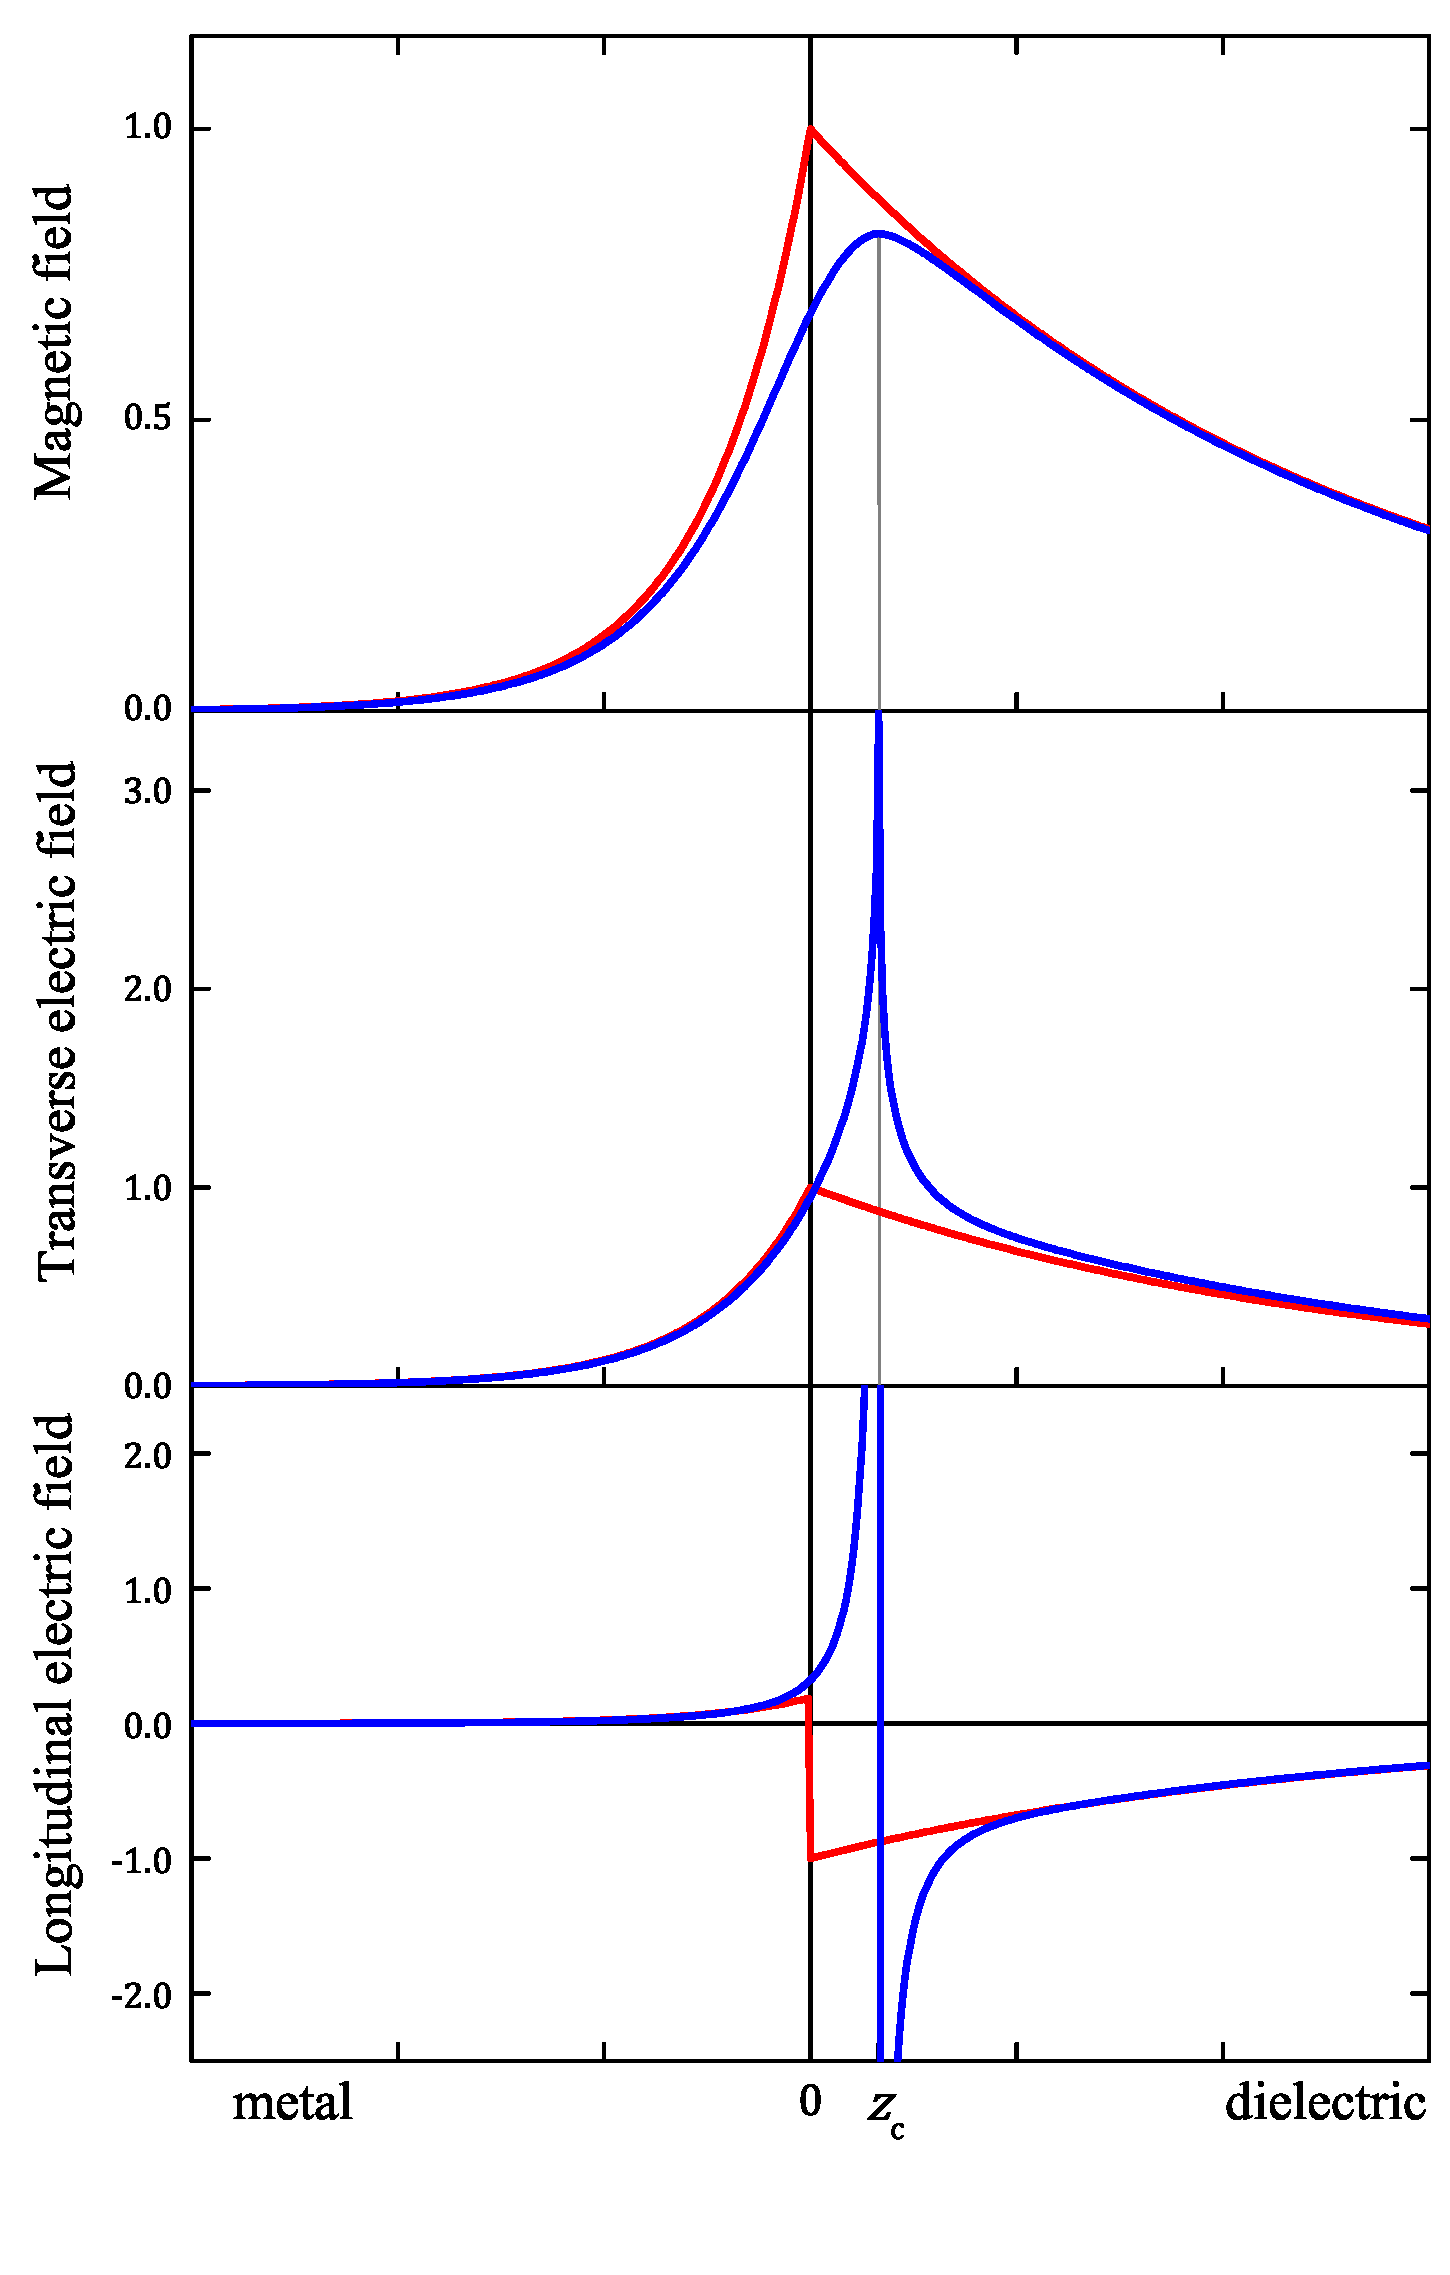
\includegraphics[width=0.75\linewidth]{EHfields.eps}
\caption{Asymptotic behavior of the SPP electromagnetic field (in a.u.) in the vicinity of the critical point $z_c$ (blue), in comparison with the case of no transition layer (red).}
\label{fig:EHfieldsPlasmon}
\end{center}
\end{figure}


Also, the~term $\omega^2/c^2$ can be neglected in comparison with $k^2/\epsilon(z)$ in the~wave equation.
With these assumptions, the~equation \cref{eq:waveeqPlasmon} can be written down as
\begin{equation}
\left(z-z_c\right)\dfrac{d}{dz}\left(\dfrac{1}{z-z_c}\dfrac{dH}{dz}\right)-k^2 H(z) = 0,
\end{equation}
and the~solution for $H(z)$, when $|z-z_c| \ll \delta$, is expressed via modified Bessel functions as
\begin{equation}
\label{eq:asymptFieldPlasmon}
H(\xi) = k\xi \left(C^{(1)} I_1\left(k\xi\right) + C^{(2)} K_1\left(k\xi\right)\right),
\end{equation}
where $\xi = z-z_c$.
The~parameter $\delta$ characterizes the~width of the~transition layer.
From \cref{eq:asymptFieldPlasmon} the~electric and magnetic fields asymptotically behave as
\begin{align}
&H(\xi) \sim 1+\dfrac12 k^2 \xi^2 \ln k\xi,\\
&E_x(\xi) \sim \dfrac{1}{\epsilon(\xi)}\dfrac{\partial H}{\partial \xi} \sim \ln k\xi,\\
&E_z(\xi) \sim \dfrac{H(\xi)}{\epsilon(\xi)} \sim \dfrac{1}{\xi}.
\end{align}
The~analysis shows that both components of the~electric field tend to infinity when $z \rightarrow z_c$ (see \cref{fig:EHfieldsPlasmon}).
Of course, such scenario is unrealistic, since there always are some inevitable losses within the~real materials and one cannot have a~pure real dielectric function, therefore the~growth of the~electric field is actually capped at a~level determined by the~imaginary part of $\epsilon(z_c)$ (see, e.g., \cite{ginzburg}).

Nevertheless, the~described electric field enhancement plays a defining role in optoelectronic devices.
In particular, the processes of spontaneous photon emission, according to the Purcell effect, occur much more often when the emitter is placed in the strong electromagnetic field \cite{schuller}.

%%%%%%%%%%%%%%%%%%%%%%%%%%%%%%%%%%%%%%%%%%%%%%%%%%%%%%%%%%%%%%%%%%%%
\section{Perturbation Theory}

Since the~thickness $\delta$ of the~ENZ transition layer is typically of the~order of several angstroms, this small parameter suggests that a~perturbation theory can be developed to calculate the~corrections to the~plasmonic spectrum.
From now on, the~problem of the~SPP propagation featuring ideal metal-dielectric interfaces will be considered an~unperturbed problem, and the~presence of the~ENZ layers will be treated as a~small perturbation.
It is easy to see, however, that a~continuous and smooth dielectric function $\epsilon(z)$ can never be represented as a~sum of the~unperturbed step-like function $\epsilon_0(z)$ and the~small correction proportional to $\delta$, which means the~wave equation \cref{eq:waveeqPlasmon} in its current form does not allow for the~perturbative approach.

\subsection{Integral Eigenvalue Problem}

With this, the~Fourier transformations of the~magnetic field of the~SPP and the~dielectric function are introduced in the~form of
\begin{equation}
\label{eq:fourierH}
H(z)~=~\int\limits_{-\infty}^{+\infty}h(p)e^{ipz}dp, \quad \textrm{where} \quad
h(p)~=~\frac{1}{2\pi}\int\limits_{-\infty}^{+\infty}H(z)e^{-ipz}dz,
\end{equation}
and
\begin{equation}
\label{eq:fourierEPS}
\frac{1}{\epsilon(z)}~=~\int\limits_{-\infty}^{+\infty}\eta(p)e^{ipz}dp, \quad \textrm{where} \quad
\eta(p)~=~\frac{1}{2\pi}\int\limits_{-\infty}^{+\infty}\frac{e^{-ipz}}{\epsilon(z)}dz.
\end{equation}
After applying the~Fourier transform to the~wave equation \cref{eq:waveeqPlasmon} as well, it takes the~following integral form:
\begin{equation}
\label{eq:inteqPlasmon}
\frac{\omega^2}{c^2}h\left(p\right)~=~\int\limits_{-\infty}^{+\infty}\left(k^2+pp'\right)\eta (p-p') h(p') dp'.
\end{equation}

Equation \cref{eq:inteqPlasmon} can be regarded as an~integral eigenvalue problem for the~plasmonic spectrum $\omega = \omega(k)$, which is valid for the~SPP on both ideal interface and interface with the~ENZ transition.
If the~integral kernel $K(p,p') = \left(k^2+pp'\right)\eta (p-p')$ satisfies the~condition $K(p,p')=K^{*}(p',p)$, which requires $\eta(p) = \eta^{*}(-p)$, the~problem is then Hermitian, and its solutions are true SPP modes with real eigenfrequencies $\omega$.

For the~unperturbed problem this is indeed the~case, because the~dielectric function $\epsilon_0(z)$ is pure real, and 
\begin{equation}
\eta_0(p)~=~\int\limits_{-\infty}^{+\infty}\frac{e^{-ipz}}{\epsilon_0(z)}dz
\end{equation}
is clearly equal to its Hermitian conjugate.

In the~presence of the~ENZ transition, the~function $1/\epsilon(z)$, while being still pure real, features a~singularity, so that in the~expression 
\begin{equation}
\label{eq:etaPlasmon}
\eta(p)~=~\dfrac{1}{2\pi} \int\limits_{-\infty}^{+\infty} \frac{e^{-ipz}}{\epsilon(z)}dz
\end{equation}
the~integration path must be curved to avoid this pole (see \cref{fig:polePlasmon}).
Therefore, the~Fourier transform of the~inverse dielectric function \cref{eq:etaPlasmon} can be rewritten as
\begin{equation}
\eta(p)~=~\dfrac{1}{2\pi} \fint\limits_{-\infty}^{+\infty} \frac{e^{-ipz}}{\epsilon(z)}dz - \frac{i}{2}\,\underset{z=z_0}{\mathrm{res}}\frac{e^{-ipz}}{\epsilon(z)},
\end{equation}
where the~integral is understood as its Cauchy principal value.
The~second term that appears due to the~singularity clearly breaks the~hermiticity of the~kernel in \cref{eq:inteqPlasmon}, and the~non-Hermitian eigenvalue problem thus results in complex eigenvalues $\omega = \omega(k) = \omega'(k) - i\omega''(k)$.

The~imaginary part of the~eigenvalue $\omega$ means that the~SPP would inevitably lose energy even if the~metal is lossless.
The~very existence of the~critical point in the~ENZ transition layer results in the~delocalization of the~plasmon energy, which therefore gradually radiates away from the~interface and depletes the~plasmon.
This novel mechanism of the~SPP decay is in some sense similar to the~Landau damping mechanism \cite{LLtom8}, since neither is due to the~electron collisions in metal, and the~difference is that the~SPP does not channel energy to the~resonant electrons, but rather couples to the~bulk plasmons in the~transition layer \cite{akimov}.

This radiative plasmonic decay was earlier reported to exist for some specially tailored dielectric permittivity profiles in a~two-layered system (see, e.g., \cite{akimov}), however, the~goal of my work is to develop a~theoretical approach that is capable of calculating the~SPP dispersion for \textit{any} function $\epsilon(z)$ and, specifically, for systems with \textit{any} number of layers, and that can also be generalized for 2D or 3D problems.

\subsection{Linear Perturbation}

Let us now seek the~solution of the~integral eigenvalue problem \cref{eq:inteqPlasmon} in the~linear order of the~perturbation theory in the~form of
\begin{equation}
\label{eq:deltaomegaPlasmon}
\omega~=~\omega(k)~=~\omega_0(k)+\Delta \omega(k),
\end{equation}
\begin{equation}
\label{eq:deltaetaPlasmon}
\eta(p)~=~\eta_0(p)+\Delta\eta(p),
\end{equation}
\begin{equation}
\label{eq:deltahPlasmon}
h(p)~=~h_0(p)+\Delta h(p),
\end{equation}
where $\omega_0(k)$, $\eta_0(p)$ and $h_0(p)$ describe the~spectrum, the~dielectric permittivity and the~magnetic field of the~SPP in the~unperturbed case, and the~corrections $\Delta \omega(k)$, $\Delta \eta(p)$ and $\Delta h(p)$ are proportional to the~small parameter $\delta$.

Substituting \cref{eq:deltaomegaPlasmon}-\cref{eq:deltahPlasmon} into \cref{eq:inteqPlasmon} and discarding quadratic over $\delta$ terms, one arrives at the~Fredholm integral equation of the~second kind for $\Delta h(p)$:
\begin{equation}
\label{eq:fredholmPlasmon}
\frac{\omega_0^2}{c^2}\Delta h\left(p\right)-\int\limits_{-\infty}^{+\infty}\left(k^2+pp'\right)\eta_0 (p-p') \Delta h(p') dp'~=~-\frac{2\omega_0\Delta \omega}{c^2}h_0\left(p\right)+F(p),
\end{equation}
where the~last term in the~right-hand side is
\begin{equation}
\label{eq:FpPlasmon}
F(p)~=~\int\limits_{-\infty}^{+\infty}\left(k^2+pp'\right)\Delta\eta (p-p') h_0(p') dp'.
\end{equation}
According to one of the~Fredholm's theorems \cite{fredholm}, the~solution of the~inhomogeneous Fredholm equation \cref{eq:fredholmPlasmon} exists if and only if the~inhomogeneous term is orthogonal to the~solution of the~adjoint homogeneous equation, i.e., if
\begin{equation}
\label{eq:fredholmtheoremPlasmon}
\int\limits_{-\infty}^{+\infty} \left(-\frac{2\omega_0\Delta \omega}{c^2}h_0\left(p\right)+F(p)\right) h_0^{*}(p) dp~=~0,
\end{equation}
where the~solution of the~homogeneous equation is nothing else but the~unperturbed magnetic field $h_0(p)$.
This orthogonality condition immediately gives the~spectrum correction $\Delta \omega$:
\begin{equation}
\label{eq:correctionPlasmon}
\dfrac{\Delta\omega}{\omega_0}~=~\frac{c^2}{2\omega_0^2}\frac{\int\limits_{-\infty}^{+\infty}F(p)h_0^{*}(p)dp}{\int\limits_{-\infty}^{+\infty}h_0(p)h_0^{*}(p)dp}.
\end{equation}
The~denominator can be further simplified using the~relation \cref{eq:fourierH}:
\begin{equation}
\int\limits_{-\infty}^{+\infty}h_0(p)h_0^{*}(p)dp~=~\frac{1}{2\pi}\int\limits_{-\infty}^{+\infty}H_0(z)H_0^{*}(z)dz~=~\frac{1}{2\pi}\int\limits_{-\infty}^{+\infty}\left|H_0(z)\right|^2 dz,
\end{equation}
which yields
\begin{equation}
\label{eq:correctionPlasmon2}
\dfrac{\Delta\omega}{\omega_0}~=~\frac{\pi c^2}{\omega_0^2}\frac{\int\limits_{-\infty}^{+\infty}F(p)h_0^{*}(p)dp}{\int\limits_{-\infty}^{+\infty}\left|H_0(z)\right|^2 dz}.
\end{equation}
In order to evaluate the~numerator, I rewrite the~expression for $F(p)$ as
\begin{equation}
\begin{aligned}
F(p)~&=~\int\limits_{-\infty}^{+\infty} dp'(k^2+pp')\Delta\eta(p-p')h_0(p') = \\
&=~\frac{1}{2\pi}\int\limits_{-\infty}^{+\infty}dp' (k^2+pp')h_0(p')\left(\int\limits_{-\infty}^{+\infty}dz e^{-i(p-p')z}\left(\frac{1}{\epsilon(z)}-\frac{1}{\epsilon_0(z)}\right)\right) = \\
&=~\frac{1}{2\pi}\int\limits_{-\infty}^{+\infty}dz \left(\frac{1}{\epsilon(z)}-\frac{1}{\epsilon_0(z)}\right)e^{-ipz} \left(\int\limits_{-\infty}^{+\infty}dp' (k^2+pp')h_0(p') e^{ip'z}\right) = \\,
&=~\frac{1}{2\pi}\int\limits_{-\infty}^{+\infty}dz \left(\frac{1}{\epsilon(z)}-\frac{1}{\epsilon_0(z)}\right)e^{-ipz} \CF(z,p),
\end{aligned}
\end{equation}
where the~order of integrations was changed to allow for the~calculation of the~inner integral over $p$. Using the~identities for the~Dirac delta function \cref{eq:app_diracdelta1}-\cref{eq:app_diracdelta4}, this inner integral, $\CF(z,p)$, is significantly simplified:
\begin{align}
\CF(z,p)~&=~\int\limits_{-\infty}^{+\infty}dp' (k^2+pp')h_0(p') e^{ip'z}~= \\
&=~\int\limits_{-\infty}^{+\infty}dp' (k^2+pp')e^{ip'z}\left(\frac{1}{2\pi}\int\limits_{-\infty}^{+\infty}dz'H_0(z')e^{-ip'z'}\right)~=\notag\\
&=~\frac{1}{2\pi} \int\limits_{-\infty}^{+\infty} dz' H_0(z')\left(\int\limits_{-\infty}^{+\infty} dp' (k^2+pp')e^{ip'(z-z')}\right)~=\notag\\
&=~\int\limits_{-\infty}^{+\infty} dz' H_0(z')\Big(k^2\delta(z-z')+i p \delta'(z-z')\Big)~=~k^2 H_0(z)-ip H_0'(z),\notag
\end{align}
Consequently, the~numerator of \cref{eq:correctionPlasmon2} is reduced to
\begin{equation}
\begin{aligned}
\int\limits_{-\infty}^{+\infty} F(p)h_0^*(p)dp~&=~\frac{1}{2\pi}\int\limits_{-\infty}^{+\infty} dp\,h_0^*(p) \left( \int\limits_{-\infty}^{+\infty}dz \left(\frac{1}{\epsilon(z)}-\frac{1}{\epsilon_0(z)}\right)e^{-ipz} \CF(z,p)\right)~= \\
&=~\frac{1}{2\pi} \int\limits_{-\infty}^{+\infty}dz \left(\frac{1}{\epsilon(z)}-\frac{1}{\epsilon_0(z)}\right) \left( \int\limits_{-\infty}^{+\infty} dp\,\CF(z,p) h_0^*(p) e^{-ipz}\right)~= \\
&=~\frac{1}{2\pi} \int\limits_{-\infty}^{+\infty}dz \left(\frac{1}{\epsilon(z)}-\frac{1}{\epsilon_0(z)}\right) G(z),
\end{aligned}
\end{equation}
with the~function $G(z)$ being
\begin{align}
&G(z)~=~\int\limits_{-\infty}^{+\infty} dp\,\CF(z,p) h_0^*(p) e^{-ipz}~=\\
&=~\int\limits_{-\infty}^{+\infty}dp \Big(k^2 H_0(z)-ip H_0'(z)\Big)e^{-ipz}\left(\frac{1}{2\pi}\int\limits_{-\infty}^{+\infty} dz'H_0^{*}(z')e^{ipz'}\right)~=\notag\\
&=~\frac{1}{2\pi} \int\limits_{-\infty}^{+\infty}dz' H_0^{*}(z')\left(k^2H_0(z)\int\limits_{-\infty}^{+\infty}dp\,e^{ip(z-z')} - iH_0'(z) \int\limits_{-\infty}^{+\infty}dp\,pe^{ip(z-z')}\right)~=\notag\\
&=~\int\limits_{-\infty}^{+\infty}dz' H_0^{*}(z')\Bigg(k^2H_0(z)\delta(z-z')-H_0'(z)\delta'(z-z')\Bigg)~=~k^2|H_0(z)|^2+|H_0'(z)|^2,\notag
\end{align}
Ultimately, the~eigenfrequency shift $\Delta\omega$ takes the~form which explicitly depends on the~magnetic field $H_0(z)$ and the~dielectric permittivities $\epsilon_0(z)$ and $\epsilon(z)$ only:
\begin{equation}
\label{eq:correctionPlasmon3}
\frac{\Delta\omega}{\omega_0}~=~\frac{c^2}{2\omega_0^2}\frac{\int\limits_{-\infty}^{+\infty}\left(\frac{1}{\epsilon(z)}-\frac{1}{\epsilon_0(z)}\right) \Big(k^2|H_0(z)|^2+|H_0'(z)|^2\Big)dz}{\int\limits_{-\infty}^{+\infty} |H_0(z)|^2 dz}.
\end{equation}


\subsection{Analysis of the Eigenfrequency Shift}

Every term in the~right-hand side of \eqref{eq:correctionPlasmon3} is pure real, yet the~integration in the~numerator results in a~complex value since one has to carefully handle the~singularities in $\frac{1}{\epsilon(z)}$, which are located at the~points where $\epsilon(z)=0$.
The~integration path must therefore be bent into the~complex $z$ plane in order to avoid the~poles $z_\sigma$, $\sigma=1,2,3,...$, distributed along the~real axis.
Curving the~integration path in the~vicinity of the~poles adds a~small imaginary part to the~function $\epsilon(z)$, and in order to perform the~integration I make use of the~following well-known identity from the~complex analysis:
\begin{equation}
\frac{1}{z-z_\sigma\pm i 0^{+}}~=~P\frac{1}{z-z_\sigma}\mp i\pi\delta(z-z_\sigma),
\end{equation}
which is a~shorthand notation for
\begin{equation}
\label{eq:plemel}
\lim_{\alpha\to 0^{+}} \int\limits_{-\infty}^{+\infty}\frac{f(z)}{z-z_\sigma\pm i\alpha}dz~=~\fint\limits_{-\infty}^{+\infty}\frac{f(z)}{z-z_\sigma}dz \mp i\pi f(z_\sigma)
\end{equation}
that is valid for an~analytic function $f(z)$.
The~integral expression in the~right is understood as its Cauchy principal value.
The~choice of the~sign of the~imaginary part for each $z_\sigma$ is determined by whether the~pole must be circumflexed in the~upper or lower semispace of the~complex plane $z$ (see \cref{fig:polePlasmon}).

%
% FIGURE #
%
\begin{figure}[ptb]
\begin{center}
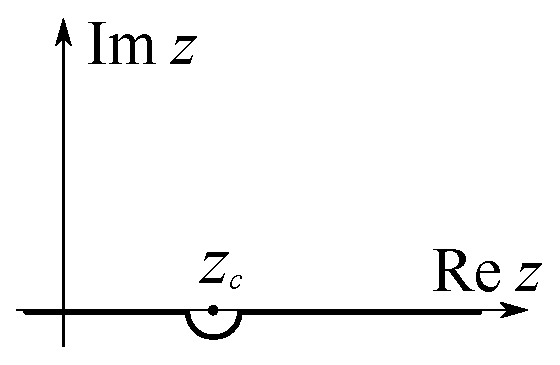
\includegraphics[width=8cm]{pole.eps}
\caption{Integration path is curved into the~lower semispace to avoid the~pole $z_c$ on the~real axis.}
\label{fig:polePlasmon}
\end{center}
\end{figure}


In general, the~pole is integrated around in a~way that is consistent with the~causality, i.e., its contribution to $\Delta\omega$ must have negative imaginary part to guarantee that the~SPP amplitude would not be exponentially increasing with time.

With that, one can separate the~real part of $\Delta\omega$:
\begin{equation}
\label{eq:correctionPlasmonRe}
\frac{\Delta\omega'}{\omega_0}~=~\frac{\re\Delta\omega}{\omega_0}~=~\frac{c^2}{2\omega_0^2}\frac{\fint\limits_{-\infty}^{+\infty}\left(\frac{1}{\epsilon(z)}-\frac{1}{\epsilon_0(z)}\right) \Big(k^2|H_0(z)|^2+|H_0'(z)|^2\Big)dz}{\int\limits_{-\infty}^{+\infty} |H_0(z)|^2 dz},
\end{equation}
from its imaginary part:
\begin{equation}
\label{eq:correctionPlasmonIm}
\frac{\Delta\omega''}{\omega_0}~=~-\frac{\im\Delta\omega}{\omega_0}~=~\frac{\pi c^2}{2\omega_0^2}\frac{\underset{\sigma}{\sum} |\epsilon'(z_\sigma)|^{-1} \Big(k^2|H_0(z_\sigma)|^2+|H_0'(z_\sigma)|^2\Big)}{\int\limits_{-\infty}^{+\infty} |H_0(z)|^2 dz}.
\end{equation}
Here I assumed the~linear behavior of the~dielectric function $\epsilon(z)$ in the~vicinity of each critical point: $\epsilon(z)\approx\epsilon'(z_\sigma)\left(z-z_\sigma\right)$, so that the~function $f(z)$ from the~identity \eqref{eq:plemel} corresponds to $\epsilon'(z)^{-1}\left(k^2|H_0(z)|^2+|H_0'(z)|^2\right)$.
The~integration path bends into the~lower semispace of the~complex plane $z$ for the~poles where $\epsilon'(z_\sigma)>0$, and into the~upper semispace otherwise. 

In addition, I emphasize that the~pure real nature of the~functions $\epsilon(z)$ and $\epsilon_0(z)$ was only used to simplify the~numerator in \eqref{eq:correctionPlasmon3}, which means the~expression for the~spectrum correction \eqref{eq:correctionPlasmon3} is valid even if the~dielectric functions are initially assumed to be complex, i.e., if they originally included the~dissipation losses as their imaginary parts.

Also, since I did not assume any particular dependence of the dielectric function on the coordinate $z$, except its linear behavior close to the critical points, the result of \cref{eq:correctionPlasmonRe} can formally take values of any sign.
This raises the question of how to limit our consideration to only those choices for $\epsilon(z)$ that are realistic and physically meaningful.
One way to do that is to obtain the plasmonic spectrum experimentally and extract the information about the sign of $\Delta\omega'$.
Knowing the sign of the left hand side of \cref{eq:correctionPlasmonRe}, one will know the sign of the integral $\fint\limits_{-\infty}^{+\infty}\left(\frac{1}{\epsilon(z)}-\frac{1}{\epsilon_0(z)}\right) \Big(k^2|H_0(z)|^2+|H_0'(z)|^2\Big)dz$ as well and thus can make an educated guess about the behavior of the dielectric function $\epsilon(z)$.

Finally, I note that in some situations it is more convenient to describe exactly the same behavior of the SPP by the pure real frequency $\omega$ and the complex wavevector $k=k(\omega)=k'(\omega)+ik''(\omega)$.
With respect to the perturbation theory, the connection between the two approaches can be established for small corrections $\Delta\omega$ and $\Delta k$ in the form of
\begin{equation}
\label{eq:omegatokPlasmon}
\Delta\omega'=-\left|\frac{d\omega}{dk}\right|\Delta k', \qquad
\Delta\omega''=\left|\frac{d\omega}{dk}\right|\Delta k'',
\end{equation}
via the group velocity $d\omega/dk$ of the unperturbed SPP mode.
Alternatively, one can explicitly use a similar perturbative approach to calculate $\Delta k$ from \cref{eq:inteqPlasmon}.

\section{SPP Dispersion}

\begin{figure}[ptb]
\subfloat{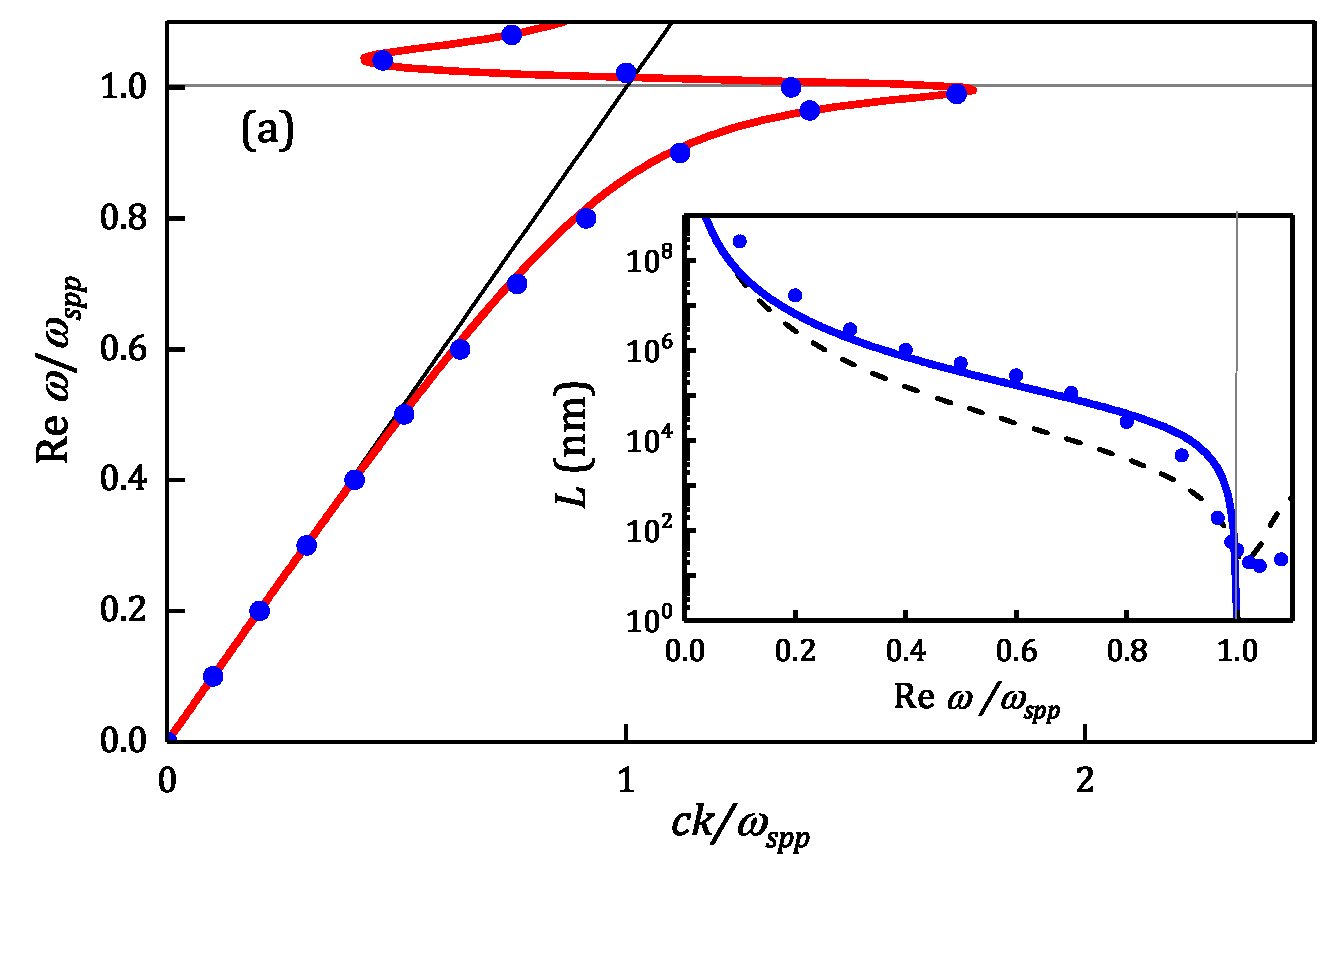
\includegraphics[clip,width=0.75\linewidth]{disp_bulk_2.eps}}

\subfloat{\includegraphics[clip,width=0.75\linewidth]{disp_thin_2.eps}}
\caption{SPP dispersion for the bulk (a) and 50nm-thick (b) silver slabs in air. The red curves and blue data points show the dispersion for the cases of ideal and realistic (with $\delta=0.02$nm) interfaces, respectively. The insets compare theoretical (blue lines) and numerical (blue data points) results for the SPP collisionless damping rates, expressed in terms of propagation length. The rate of Joule losses is shown with dashed black lines.}
\label{fig:dispersionPlasmon}
\end{figure}

Validating the theoretical predictions requires performing a number of numerical simulations.
In every simulation, I model the continuous metal-dielectric transitions with the dielectric function
\begin{equation}
\label{eq:epsilonContinuous}
\epsilon(z)~=~\epsilon_d + \frac{\epsilon_m-\epsilon_d}{1+e^{z/\delta}},
\end{equation}
where the parameter $\delta$ defines the transition layer thickness (see \cref{fig:profilePlasmon}).

Here I compare the predictions of the perturbation theory with the SPP dispersion corrections calculated numerically.
In order to do that, I numerically find the eigenvalues $\omega$ of the wave equation \cref{eq:waveeqPlasmon} for given wavevector $k$ and permittivity $\epsilon(z)$ as follows.
The eigenvalue $\omega$ is initially set equal to that of the unperturbed spectrum: $\omega=\omega_0(k)$.
The wave equation is then independently solved in the two regions, $z>0$ and $z<0$, with the specified asymptotic behavior imposed towards both infinities according to $|H(z)| \underset{z\rightarrow \pm\infty}{\longrightarrow} 0$.
The two solutions are renormalized to satisfy the magnetic field continuity $H(0^{+})=H(0^{-})$, and the value of the goal function $|E_x(0^{+})-E_x(0^{-})|$ is computed.
If the obtained value is lower than some set threshold, the longitudinal electric field $E_x(z)$ is considered to be continuous as well and the eigenvalue $\omega$ is thus found; otherwise, the optimization procedure is run to minimize the goal function, sweeping over the region of complex $\omega$.

I calculated the SPP dispersion for the cases of bulk and 50nm-thick silver slabs surrounded by air (see \cref{fig:dispersionPlasmon}).
For the dielectric permittivity of silver, I used the experimental data from \cite{johnson} that was fit by the generalized Lorentz-Drude model as described in \cite{rakic} (see Appendix~\ref{appSilver} for details).
Here $\delta=0.02$ nm, so that the thickness of the ENZ layer is on the order of 1 \AA.

In both cases, there were no drastic changes to the real part of the SPP dispersion due to including the ENZ transition layer into consideration, as seen from the main panels in \cref{fig:dispersionPlasmon}.
Instead, of particular interest are the results shown in the insets, where the imaginary part of $\omega$ is plotted in terms of the SPP propagation length.
The propagation length $L$ measures the distance over which the plasmon energy decreases by a factor of $e$ and can be expressed in terms of $\omega''$ as $L=(2 \omega'')^{-1} |d\omega/dk|$.

For the bulk sample, there is a good agreement between the theoretical and numerical estimations of the SPP decay rate that is only due to the SPP radiation through the critical point where $\epsilon(z)=0$.
When approaching the plasmon resonance frequency, the perturbation theory predicts much faster decay than the numerical calculation.
This happens because at high frequencies, one may no longer assume the perturbation to be small (the condition $k\delta \ll 1$ is not valid anymore), and the perturbation theory is no longer applicable.

For the thin film sample, there is also a good agreement for the high-frequency SPP mode, while the solution for the low-frequency SPP mode either under- or overestimates the numerically simulated propagation length, which is probably due to the perturbation theory exceeding its validity region.

For the reference, both insets also display the SPP propagation length that is only due to the Joule losses in metal in the Drude model.
This dissipative decay rate grows with frequency considerably slower than the decay rate due to the SPP radiative losses, and above the certain frequency the radiative decay becomes the dominant channel for energy dissipation.



\section{Excitation of SPP in the Transition Layer}

\subsection{Experimental Motivation}

\begin{figure}[ptb]
\begin{center}
\subfloat{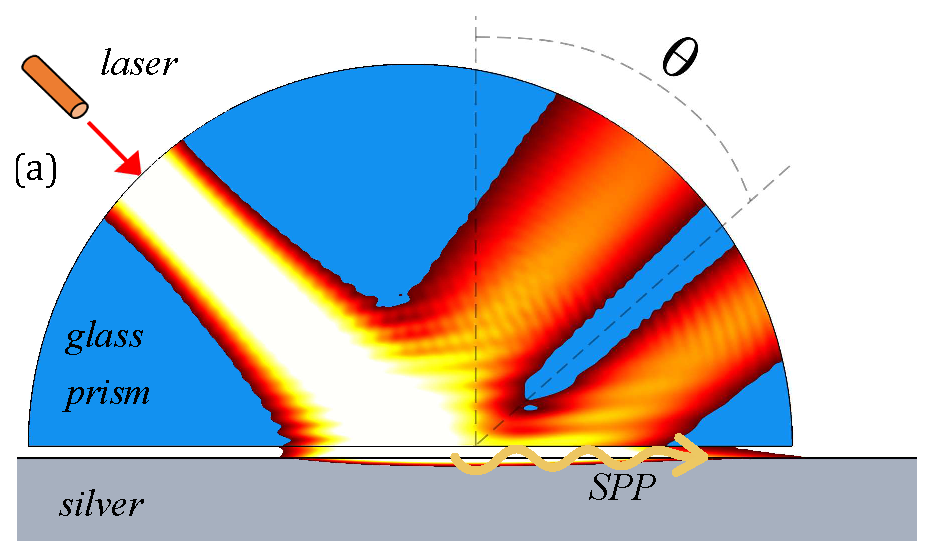
\includegraphics[clip,width=0.8\linewidth]{otto2.eps}}\\[1.0cm]
\subfloat{\includegraphics[clip,width=0.8\linewidth]{kret2.eps}}
\caption{Excitation of the SPP (a) on the silver slab in Otto configuration and (b) on the thin film in Kretschmann configuration \cite{raether}.}
\label{fig:ottosetupPlasmon}
\end{center}
\end{figure}

The two other simulations that were performed using the finite-element method modeled the excitation of the SPP by light.
In experiment such scenario is typically realized in either Otto or Kretschmann configuration \cite{raether}, where a laser beam propagates through a glass prism and is incident at an angle on a plasmonic sample.
The material of the prism must be more optically dense than the dielectric of the sample, which is a necessary condition that allows matching between the SPP wavevector and the parallel to the sample component of the wavevector of the laser.
In the absence of the prism the SPP excitation would never occur as the SPP wavevector $k_{SPP} > \omega/c$ would always be larger than the wavevector of light $k = \omega/c$.
The latter expresses the fact that SPPs propagate with the phase speed that is lower than the speed of light in corresponding dielectric medium.

\cref{fig:ottosetupPlasmon}(a) shows the excitation of SPP in the Otto configuration, which differs from the Kretschmann configuration on \cref{fig:ottosetupPlasmon}(b) only in the position of the prism.
Namely, in the Kretschmann configuration the prism sits on top of the metallic part of the plasmonic sample and the SPP is excited on the interface inside the sample, whereas in the Otto configuration the prism is separated from the sample by the air (or other dielectric) gap which leads to the SPP excitation along the interface between the air and the sample.
In the latter case the SPP may also be excited on the other interface of metal, provided the sample is relatively thin.
If it were thick, though, no excitation would reach that other interface due to the exponential weakening of the electromagnetic field as it propagates across the metallic layer.

Now, since one must also incorporate into setup the ability to control the width of the transition layer on the metal-dielectric interface by applying external DC field, the real sample would actually be a multi-layered structure.
Besides the possible dielectric substrate and index-matching layers, there have to be two outer layers serving as electrodes.
Such layers must be transparent for light, but still be able to conduct electricity.
Even though it is possible to find material that satisfies both these requirements (indium tin oxide, or ITO), one would need to carefully select the laser wavelength for the experiment in order to minimize losses in the auxiliary layers without getting too far from the SPP resonance.

It is for certain, however, that for the experiment with the bulk (thick) metallic sample only the Otto configuration is viable.
On the contrary, exciting SPPs on a thin metallic film benefits from the Kretschmann configuration as it becomes possible to negate the unavoidable issues with the uneven contact between the prism and the sample due to the surface roughness, e.g., by submerging the sample in the index matching liquid.


\subsection{Models for FEM Numerical Simulation}

For the purpose of comparing the theoretical results \cref{eq:correctionPlasmonRe} and \cref{eq:correctionPlasmonIm} derived earlier with the possible outcome from the envisioned experiment, I simulate the SPP excitation on the air-silver interface using the following two models.

In the first model, the SPP is excited on top of the bulk silver slab in Otto configuration (see \cref{fig:ottosetupPlasmon}(a)).
In this setup, the laser light is illuminating the hemicylindrical glass prism and is totally internally reflected from the glass-air interface.
However, the evanescent electromagnetic field is still able to reach across the thin (125nm) air gap and excite the plasmon on the metal surface.
%
In the second model, the bulk silver slab is replaced with a thin silver film and the air gap is removed (Kretschmann configuration, see \cref{fig:ottosetupPlasmon}(b)), allowing the excitation of the plasmonic mode at the air-silver interface.

The laser wavelength is $\lambda=370$nm, which is chosen to be close to the SPP resonance.
I define the resonant frequency $\omega_{spp}$ by the condition $\re \epsilon_m(\omega_{spp}) + \epsilon_d = 0$, which makes $\omega_{spp}$ correspond to the wavelength of approximately 331nm.
The actual plasmonic resonance is observed at a slightly lower frequency due to the dissipation in metal.
The refractive index of the prism is set to $n=1.75$ (a sapphire prism).


\subsection{Simulation Results}

\begin{figure}[ptb]
\subfloat{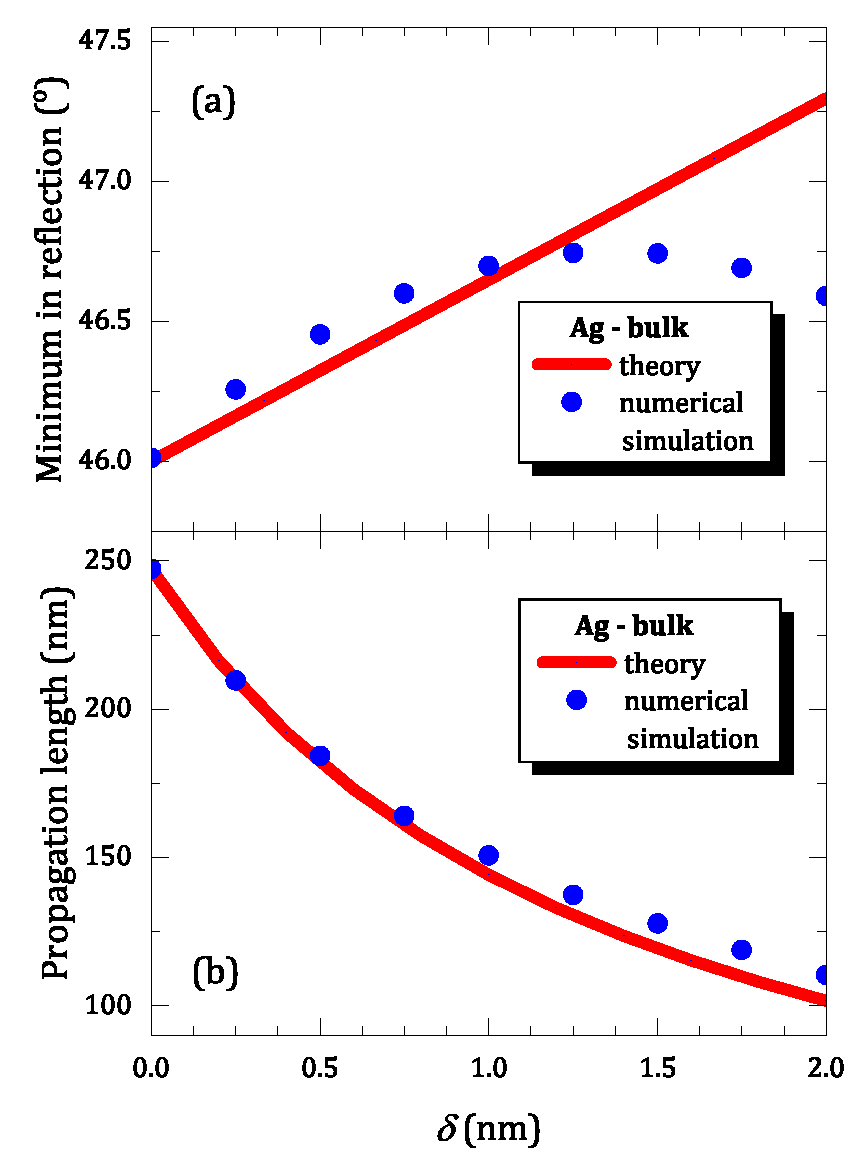
\includegraphics[clip,width=0.48\linewidth]{minpos_bulk.eps}}
\subfloat{\includegraphics[clip,width=0.48\linewidth]{minpos_thin.eps}}
\caption{Angular positions of the reflected intensity minimum (a,c) and propagation lengths (b,d) for the SPP on the bulk (left panels) and 50nm-thick (right panels) silver slabs as a function of $\delta$. Red curves represent the theoretically calculated dependence and blue data points correspond to the numerical simulations. The results for the ideal interface are included as the data at $\delta=0$.}
\label{fig:minposPlasmon}
\end{figure}

In order to excite the SPP on the air-silver interface, the plasmon wavevector $k=k(\omega)$ must match the parallel to the interface component of the wavevector of the laser light: $k(\omega)=n\omega/c \sin\theta$.
When this condition is satisfied, there will be a minimum in reflection at exactly the direction given by angle $\theta$ (see \cref{fig:ottosetupPlasmon}).
%
For the chosen parameters, the minimum in reflection in the case with bulk sample is observed for $\theta=46.0^{\circ}$, and in the case of  the 50nm-thick film the minimum is at $\theta=40.0^{\circ}$ and $\theta=55.6^{\circ}$ indicating the excitation of the plasmonic mode at the lower (air-silver) interface.

With that, I impose the continuous dielectric permittivity \cref{eq:epsilonContinuous} on the air-silver interfaces and detect how the minimum in reflection shifts its angular position and how the plasmon propagation length changes when varying the parameter $\delta$.

\cref{fig:minposPlasmon} shows the results obtained for both samples.
The minimum in reflection was identified by the angle $\theta$ at which the intensity of the reflected laser light along the circular surface of the prism is the lowest.
As for the propagation length, its evaluation requires extracting the dependence of the SPP intensity on the coordinate along the interface.
The logarithm of the intensity is expected to decay linearly with the distance, which follows from the relation $I(x)=I_0 e^{-2x/L}$.
Then, if one fits a linear function to such data and finds its slope, the propagation length is calculated as $L=-2/\mathrm{slope}$.

The data points from the numerical simulation indicate that the SPP propagation length is significantly reduced when increasing $\delta$, and the minimum in reflection shifts towards the larger angles $\theta$ which means the SPP dispersion shifts towards higher wavevectors $k$ for a given frequency $\omega$.
The same can alternatively be thought of as a red-shift of the SPP eigenfrequencies $\omega$ for a given wavevector $k$.
The theoretical results for the propagation length $L=(2\omega'')^{-1} |d\omega/dk|$ shown in \cref{fig:minposPlasmon} are calculated based on \cref{eq:correctionPlasmonIm}, while the resonant excitation condition $k(\omega)=n\omega/c \sin\theta$ together with \cref{eq:omegatokPlasmon} gives the angular shift $\Delta\theta=\Delta k'/k \tan\theta=-\Delta\omega'/k |d\omega/dk|\tan\theta$.

The theoretical calculations demonstrate good agreement with the numerical data, except for $\delta>1$nm, when the numerically simulated angular position of the minimum actually starts decreasing and the perturbation theory results become invalid.
The reason for it is the strong modification of the SPP spectrum for large $\delta$.
Namely, increasing the SPP damping always implies a reduction of the wavevector of the plasmon at the resonant frequency $\omega_{spp}$, and because of the significant SPP damping due to radiation losses the SPP excitation indeed occurs for smaller incident angle $\theta$.

Another factor to mention is the influence of the prism, which explicitly allows the SPP to leak out through itself and therefore introduces more modifications to the SPP spectrum which are unaccounted for by the~perturbation theory.
In the real experiment, there may also arise additional issues with the sample heating during the SPP excitation, the possible dielectric breakthrough and the charge leakage under influence of the applied DC electric field.

%%%%%%%%%%%%%%%%%%%%%%%%%%%%%%%%%%%%%%%%%%%%%%%%%%%%%%%%%%%%%%%%%%%%
\section{Summary}

This chapter comprises of the comprehensive theoretical and numerical studies of the SPP propagation in layered systems along the interfaces featuring epsilon-near-zero transition regions.
I developed the novel integral approach to the SPP eigenvalue problem, which is then applied to calculate the linear correction to the SPP spectrum.
The obtained correction describes the spectrum difference with respect to the setting with "ideal" interfaces, i.e., where the transition layer is regarded as infinitesimally thin.
I demonstrated that this correction is essentially complex, which means that even in a lossless environment the plasmon acquires a nonzero dissipation rate.
In other words, the critical point within the epsilon-near-zero region opens a new energy decay channel for the SPP.
This decay is due to neither the electron collisions in metal nor the metal surface roughness, as these factors were intentionally eliminated from the system.
However, the SPP now has the possibility to excite the bulk plasmons via the critical point.
The SPP thus eventually radiates its energy away from the interface, and adjusting the transition layer width presents a new means of manipulating the SPP resonant frequency as well as its propagation length.
The obtained general expression for the spectrum correction is valid for the arbitrary dielectric function profile, and the proposed analytical approach may easily be extended to address more complicated geometries, in particular, cylindrical or spherical layered structures.

I also numerically simulated the SPP propagation and excitation on top of the two silver samples --- bulk metal and thin film, ---  and computed the changes to the plasmonic dispersion caused by the smooth transition of the dielectric function between the media.
The theoretical predictions agree well with the numerical simulation for frequencies which are not too close to the SPP resonance.

These findings are of particular importance for designing the plasmonic-based optical devices which employ SPPs for the photon emission enhancement and for near-field imaging applications.

%%% Local Variables: 
%%% mode: latex
%%% TeX-master: "dissertation"
%%% End: 
